%-------------------------------------------------------------------------------
%                            BAB III
%               		METODOLOGI PENELITIAN
%-------------------------------------------------------------------------------
\fancyhf{} 
\fancyfoot[C]{\thepage}
\chapter{METODOLOGI PENELITIAN}

\section{Waktu dan Lokasi Penelitian}
Penelitian ini akan bertempat pada Gedung A Fakultas Matematika dan Ilmu Pengetahuan Alam. Waktu yang dibutuhkan agar penelitian ini dapat diimplementasikan adalah 5 bulan terhitung dari Agustus 2022 hingga Desember 2022.

\section{Alat dan Bahan}
Alat dan Bahan yang akan digunakan pada penelitian ini terdiri dari beberapa perangkat keras (\textit{Hardware}) dan perangkat lunak (\textit{Software}) yang dijabarkan sebagai berikut:

\begin{enumerate}
\item Perangkat Keras
	\begin{itemize}
	\item Laptop Acer Aspire E5-475g dengan RAM 16GB, Intel Core i5-7200U 2.5GHz, Nvidia GeForce 940MX 2GB, \textit{Harddisk} (HDD) 1500Gb, \textit{Solid State Drive} (SSD) 250GB.
	\item \textit{Smartphone} Xiaomi Poco F3 dengan RAM 6GB, \textit{Internal Storage} 128GB.
	\item \textit{Personal Computer} dengan AMD Ryzen 7 2700x, RAM 16GB, Nvidia GeForce RTX 2080 8GB, \textit{Solid State Drive} (SSD) 500GB.
	\item \textit{Beacon Bluetooth}.
	\end{itemize}

\item Perangkat Lunak
	\begin{itemize}
	\item Windows 11 Pro
	\item Linux Ubuntu 20.04.1 LTS
	\item Android Studio 2021.2.1.15
	\item Visual Studio Code
	\item Figma
	\item Notion
	\item Vosk API
	
	\end{itemize}
\end{enumerate}


\newpage
\section{\textit{Roadmap} Penelitian}
\textit{Roadmap} penelitian merupakan diagram yang menggambarkan rangkaian beberapa penelitian yang saling berkesinambungan dalam rentang waktu tertentu. \textit{Roadmap} penelitian biasa dibuat untuk memberikan batasan kepada peneliti agar menghindari pengamatan yang tidak perlu dan fokus terhadap bagian penelitiannya saja. Pada penelitian ini dibagi ke dalam 2 fase. Fase pertama pada tahun 2019 memiliki fokus penelitian pada \textit{indoor localization} dengan menggunakan \textit{Bluetooth Low Energy} (BLE) dan menggunakan \textit{Wireless Local Area Network} (WLAN) dapat dilihat gambar \ref{img:fase1}. Pada fase kedua pada tahun 2020 lebih berfokus pada penelitian \textit{Indoor Localization} dengan menggunakan BLE. Penelitian ini terletak pada fase 2 di tahun 2020 dengan topik utama yaitu Aplikasi Navigasi \textit{Indoor} dengan sub topik untuk pengguna Tunanetra. Penelitian ini memiliki batasan berupa pembangunan aplikasi \textit{mobile} untuk \textit{Route Guidance} untuk Tunanetra, seperti yang ditunjukkan pada gambar \ref{img:fase2} dengan kata yang dicetak tebal berwarna merah sebagai berikut.


\begin{figure}[H]
  \begin{adjustbox}{addcode={\begin{minipage}{\width}}{\caption{%
      \textit{Roadmap} Penelitian Fase 1
      }\label{img:fase1}\end{minipage}},rotate=90,center} %label gambar simpen disetelah capt
      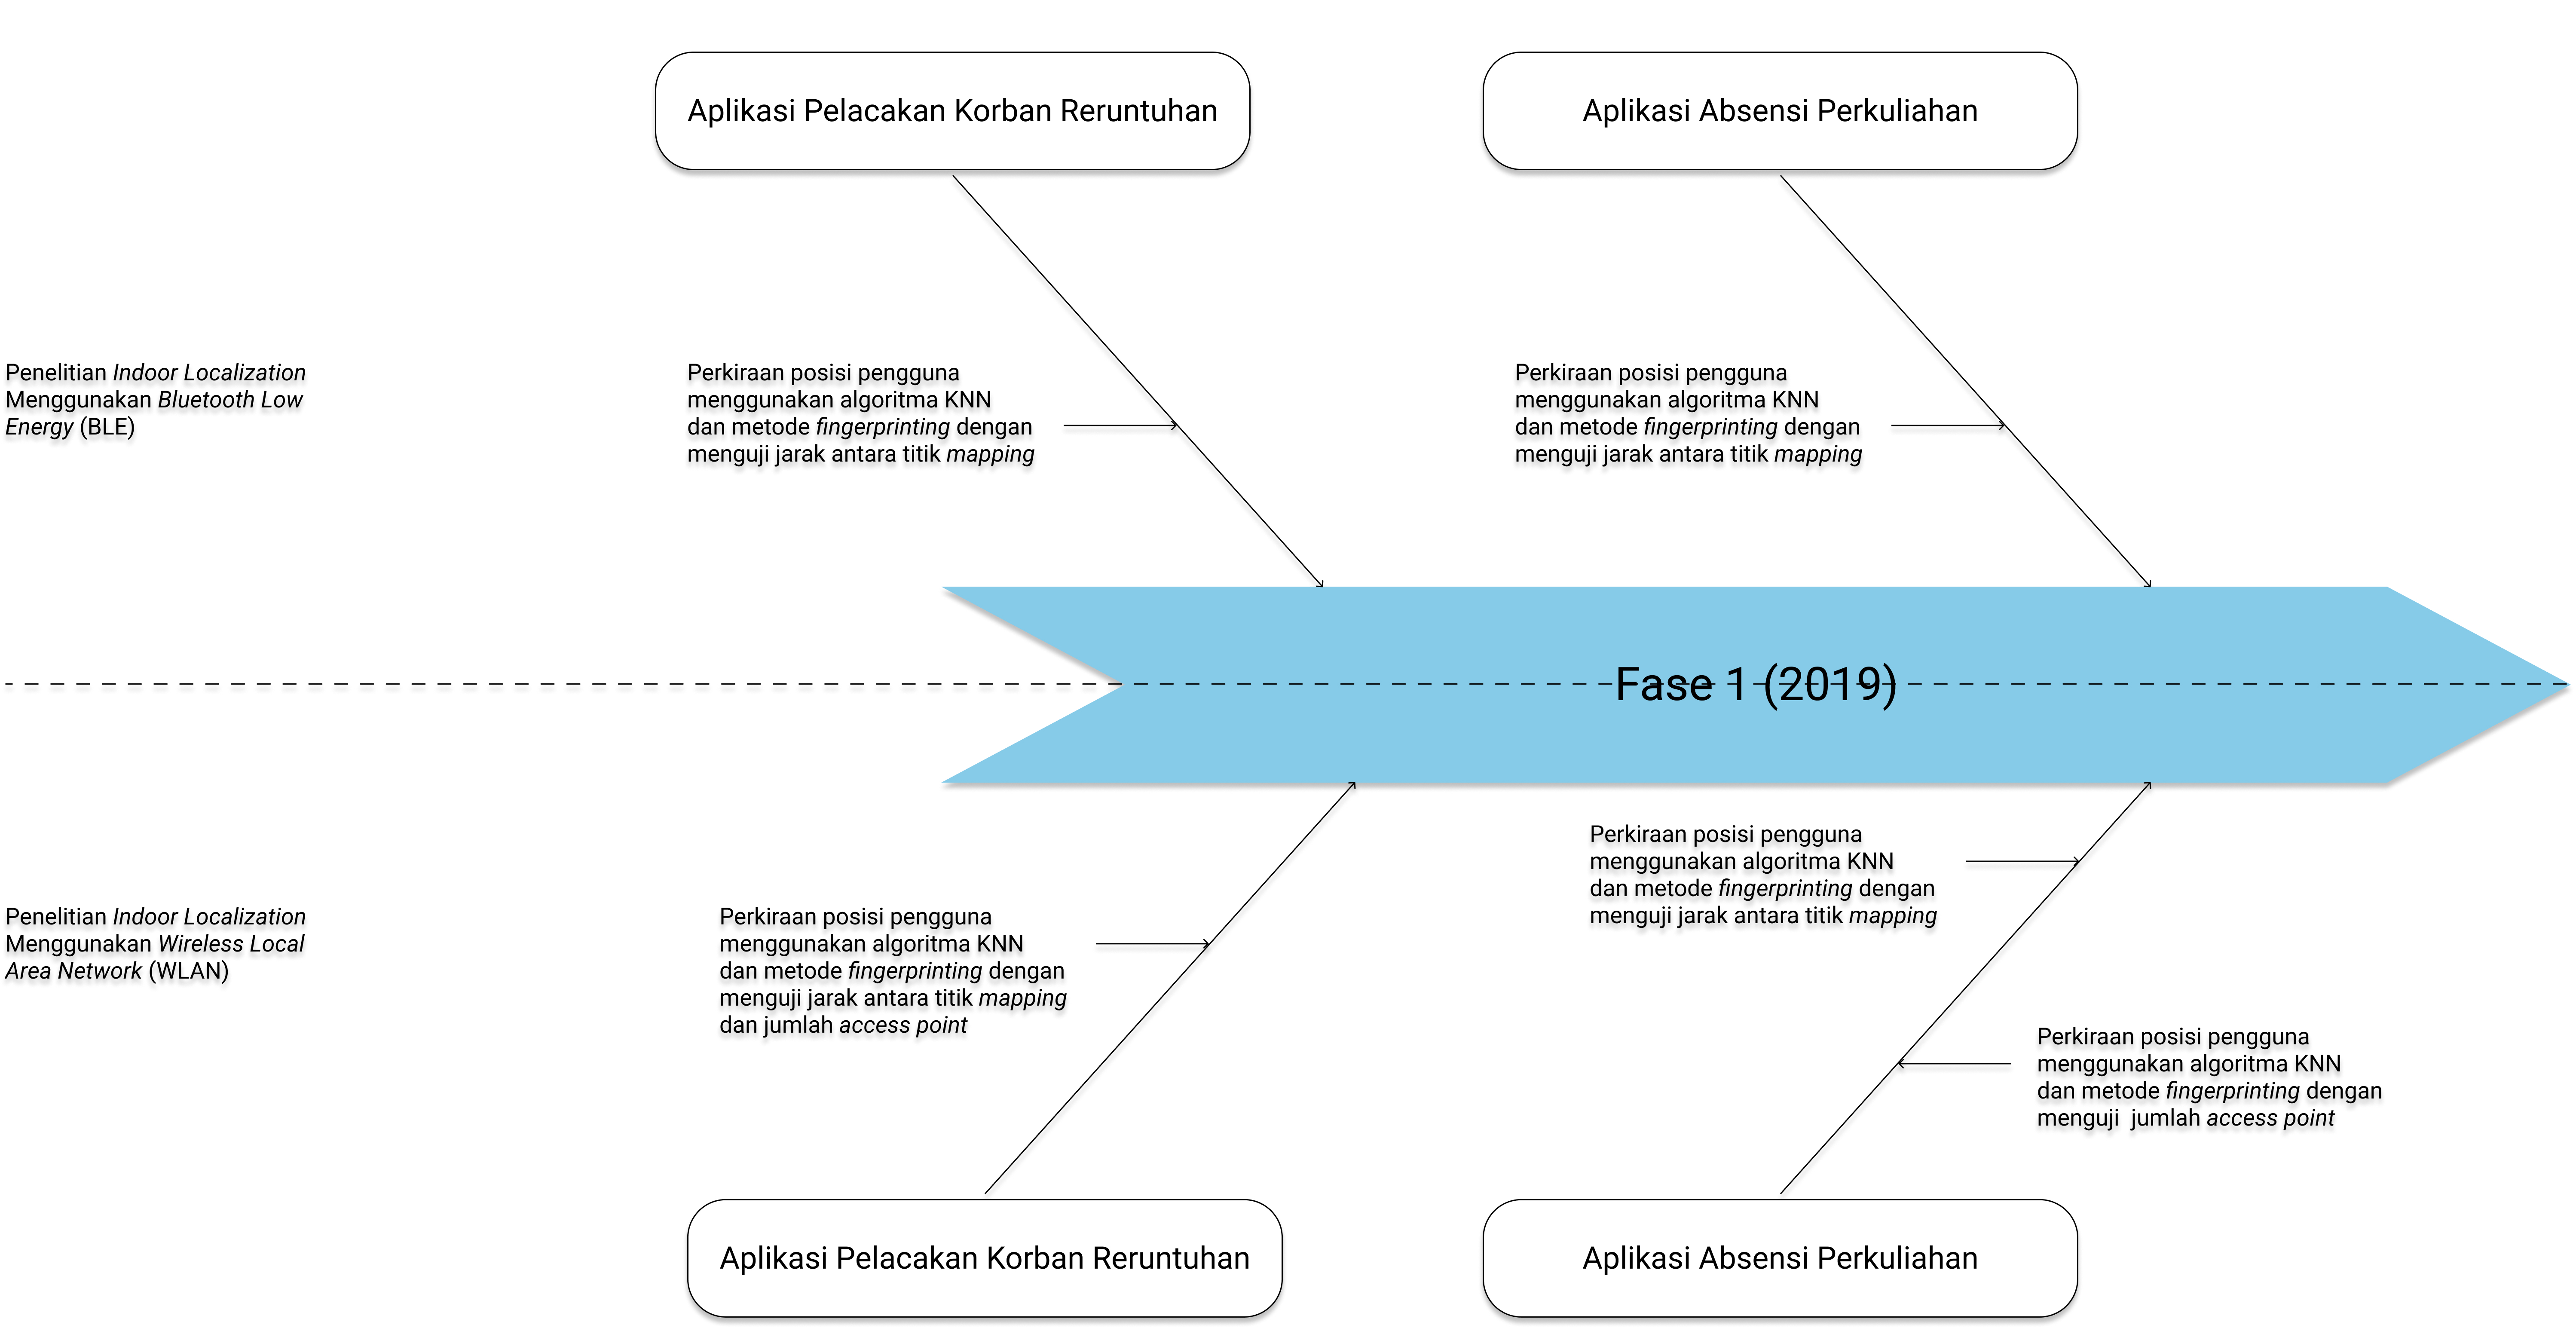
\includegraphics[scale=.3]{gambar/bab3/rp_fase1}%
  \end{adjustbox}
\end{figure}

\fancyhf{} 
\fancyfoot[R]{\thepage}

\begin{figure}[H]
  \begin{adjustbox}{addcode={\begin{minipage}{\width}}{\caption{%
      \textit{Roadmap} Penelitian Fase 2
      }\label{img:fase2}\end{minipage}},rotate=90,center}
      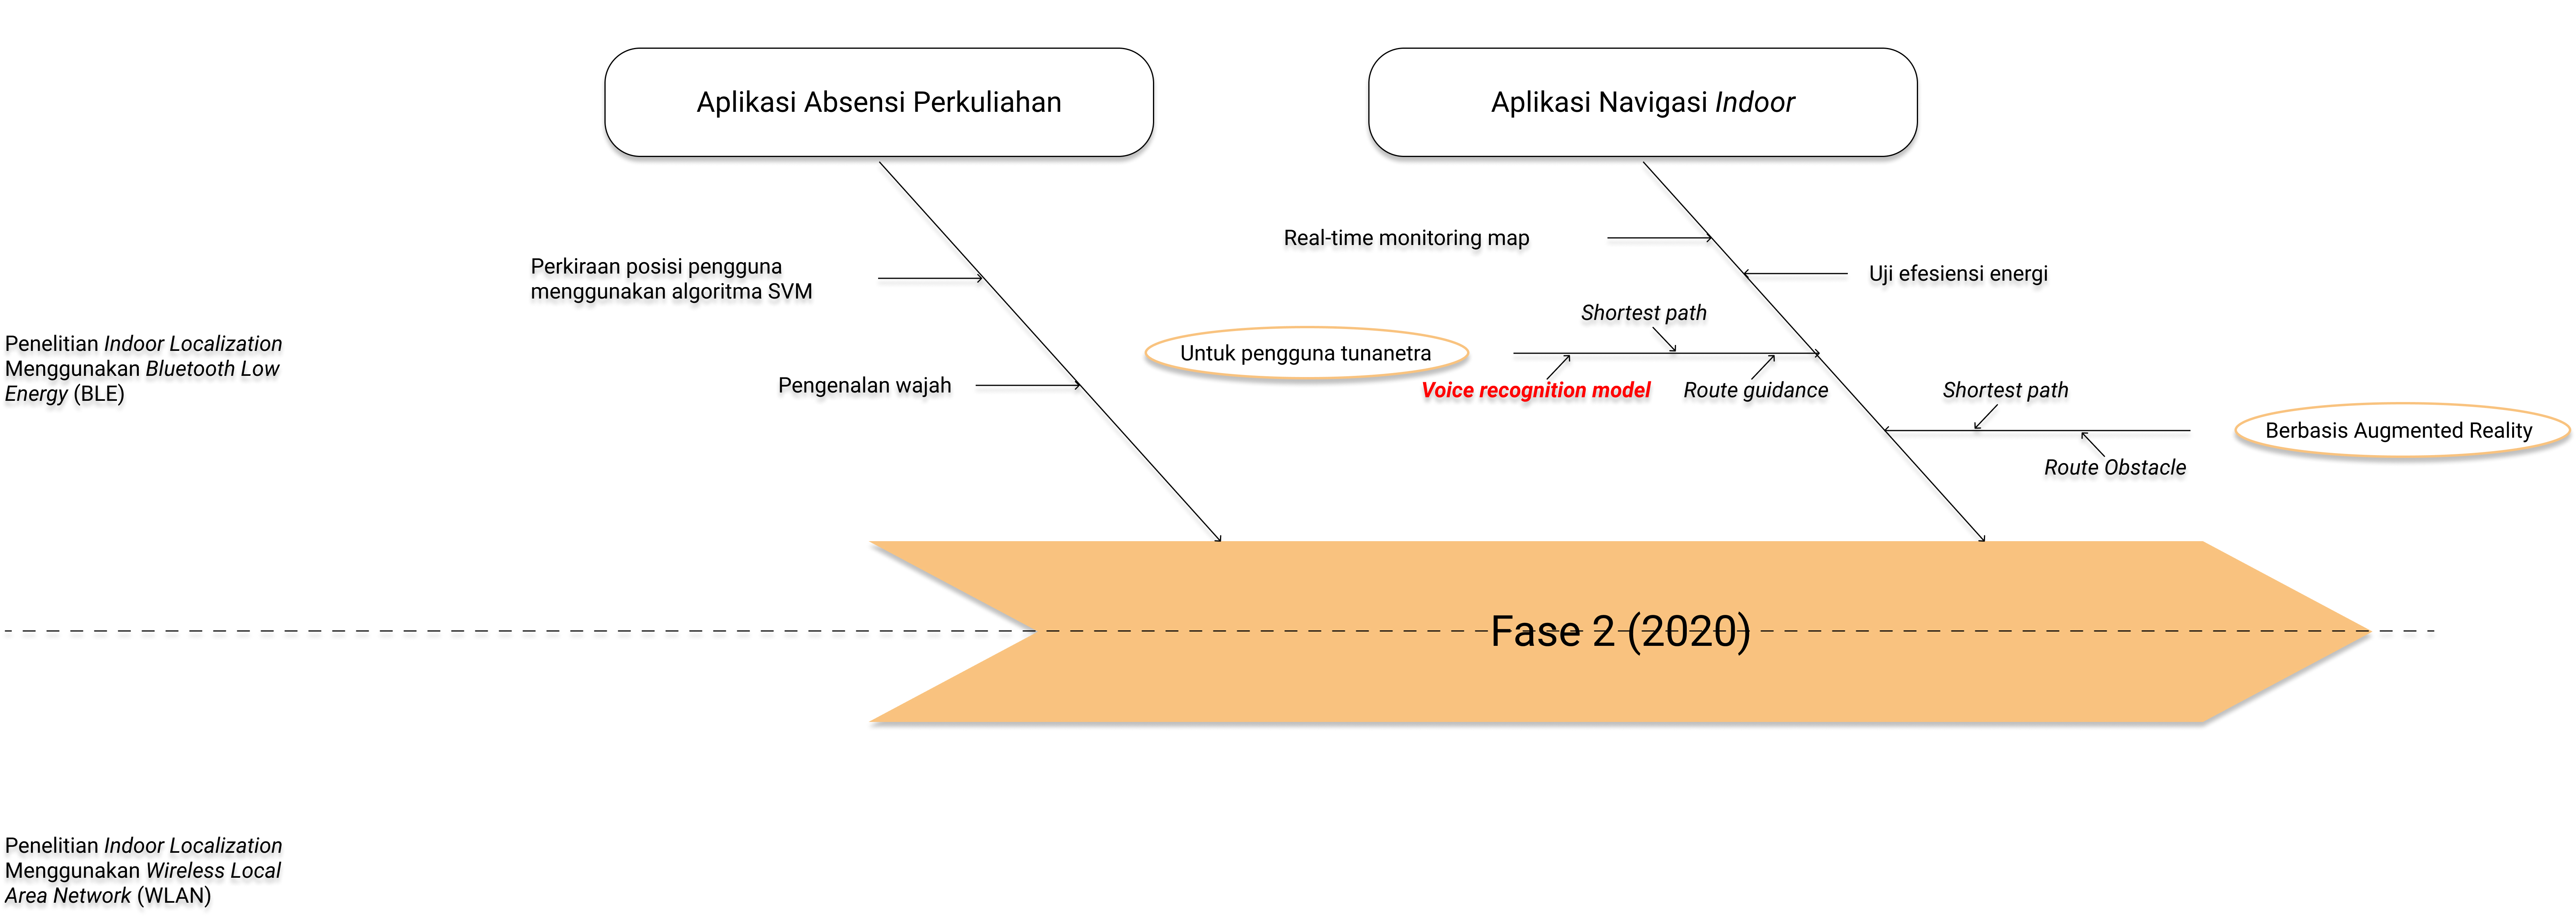
\includegraphics[scale=.6]{gambar/bab3/rp_fase2}%
  \end{adjustbox}
\end{figure}

\fancyhf{} 
\fancyfoot[R]{\thepage}

\section{Metode Penelitian}
Metode penelitian yang dilakukan dalam penelitian ini ditunjukkan pada Gambar \ref{img:diagram_alir_penelitian}.

\begin{figure}[H]
\centering
{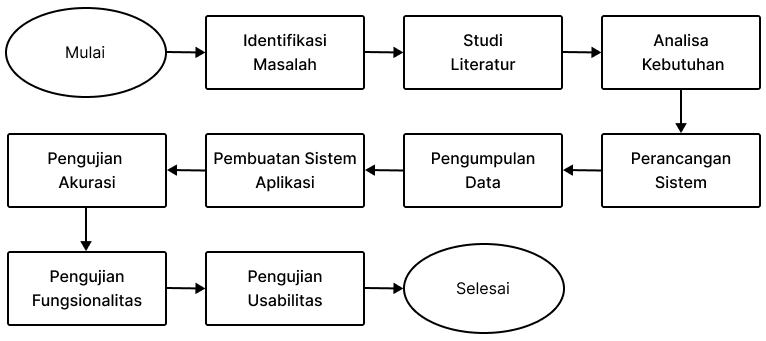
\includegraphics [scale= 0.7]{gambar/bab3/diagram_alir}}
\caption{Diagram Alir Penelitian}
\label{img:diagram_alir_penelitian}
\end{figure}

\fancyhf{} 
\fancyfoot[R]{\thepage}

\subsection{Identifikasi Masalah}
Tahapan ini merupakan tahapan yang dilakukan untuk mengidentifikasi masalah pada lingkungan yang berhubungan dengan aplikasi yang akan dibuat baik secara langsung maupun tidak langsung dan menjadi landasan mengapa aplikasi ini harus dibuat. Masalah-masalah yang berhasil di identifikasi adalah sebagai berikut:

\begin{enumerate}
\item Kebutuhan Fungsional
Kebutuhan fungsional mendefinisikan fungsionalitas sistem. Kebutuhan fungsional dari identifikasi masalah yang telah dilakukan adalah sebagai berikut:

\begin{itemize}
\item Melakukan proses pemanduan kepada pengguna secara \textit{background process} dengan bantuan \textit{speech command recognition} dan \textit{route guidance} dengan aplikasi berbasis Android.

\item Menampilkan prediksi lokasi pengguna serta rute terbaik menuju ke lokasi tujuan pengguna.

\end{itemize}

\item Kebutuhan Non-Fungsional
Kebutuhan non-fungsional memastikan batasan eksternal yang harus dipenuhi oleh sistem. Batasan-batasan tersebut antara lain:

\begin{itemize}
\item Proses pemanggilan aplikasi dimulai dengan memanggil \textit{hotword}.

\item Proses pencatatan dan penentuan lokasi dilakukan secara berkala dalam interval yang sesingkat-singkatnya.

\item Hanya dapat melakukan proses pemanduan rute apabila \textit{Bluetooth} pada perangkat hidup dan terhubung dengan \textit{Beacon}.

\item Sistem hanya dapat mendeteksi lokasi pengguna di dalam gedung yang telah di petakan terlebih dahulu.

\end{itemize}

\end{enumerate}

%%%%%%%%%%%%%%%%%%%%%%%%%%%%%%%%%%%%%%%%%%%
\subsection{Studi Literatur}
Studi literatur digunakan sebagai bahan referensi selama proses penelitian. Studi literatur dilakukan dengan cara mencari situs \textit{website} dan jurnal-jurnal terkait tentang penelitian, baik jurnal nasional maupun internasional, buku-buku yang telah diterbitkan, serta situs-situs internet yang berkaitan dengan permasalahan yang dikaji dalam penelitian. Studi literatur dapat dikembangkan untuk menyempurnakan kekurangan dari penelitian sebelumnya.

%%%%%%%%%%%%%%%%%%%%%%%%%%%%%%%%%%%%%%%%%
\subsection{Perancangan Sistem}
Tahap perancangan sistem ini meliputi perancangan alur kerja sistem yang berfungsi untuk memastikan sistem yang dibangun dapat digunakan secara baik oleh pengguna. Tahap perancangan sistem ini terbagi menjadi beberapa bagian yaitu diagram Use Case , Diagram Deployment, alur kerja sistem, \textit{Flow Diagram} dan desain prototipe berdasarkan analisa kebutuhan yang telah dijabarkan. Berikut ini merupakan tahapan tersebut:



\begin{enumerate}
\item \textit{Use Case Diagram}
\par \textit{Use Case Diagram} merupakan gambaran interaksi antara pengguna dan sistem. Pengguna dari sistem yang akan dibangun ini adalah Tunanetra dan pengunjung gedung FMIPA USK. \textit{Use Case Diagram} dari sistem ini dapat dilihat pada Gambar \ref{img:use_case_diagram}

\begin{figure}[H]
\centering
{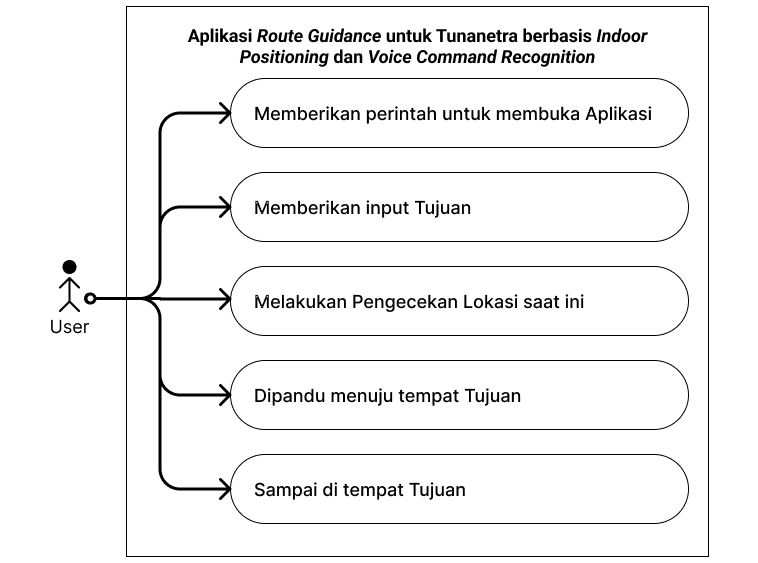
\includegraphics [width = 12cm, height= 10cm]{gambar/bab3/use_case_diagram}}
\caption{\textit{Use Case Diagram}}
\label{img:use_case_diagram}
\end{figure}

\newpage
\item \textit{Deployment Diagram}
\par \textit{Deployment Diagram} merupakan gambaran hubungan antara perangkat lunak dan perangkat keras yang digunakan dalam sebuah sistem. Seperti yang telah disebutkan sebelumnya, penelitian ini merupakan bagian dari penelitian lain yang saling terintegrasi sehingga tidak semua \textit{node} dalam diagram menjadi fokus dalam penelitian ini. Bagian dalam diagram yang menjadi jangkauan dari penelitian ini ditandai dengan warna biru seperti yang ditunjukkan pada Gambar \ref{img:deployment_diagram}

\begin{figure}[H]
\centering
{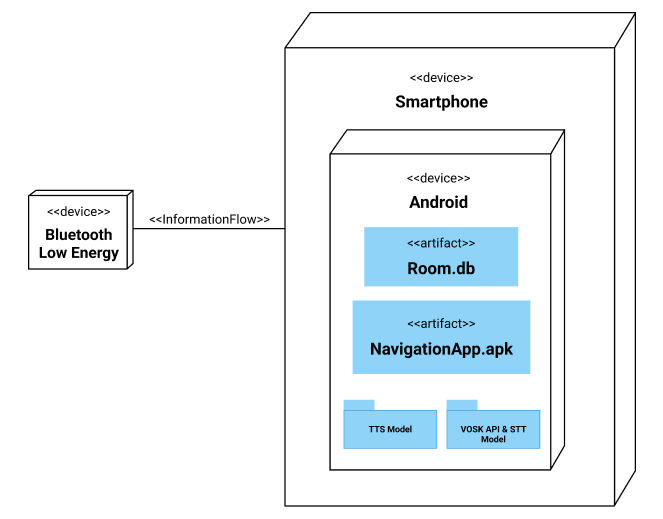
\includegraphics [width = 10cm, height= 8cm]{gambar/bab3/deployment_diagram}}
\caption{\textit{Deployment Diagram}}
\label{img:deployment_diagram}
\end{figure}


\newpage
\item Alur Kerja Sistem

\par Alur kerja sistem merupakan langkah-langkah yang dilalui sistem hingga fungsionalitas sistem dapat dimanfaatkan oleh pengguna. Alur kerja sistem ini dapat dilihat pada Gambar \ref{img:alur_kerja_sistem}

\begin{figure}[H]
\centering
{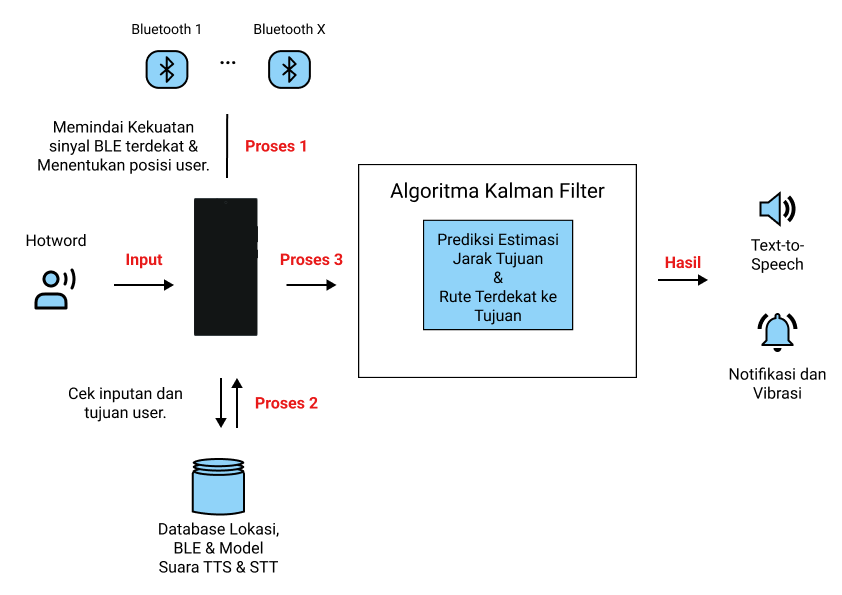
\includegraphics [scale = 0.5]{gambar/bab3/alur_kerja_sistem}}
\caption{Alur Kerja Sistem}
\label{img:alur_kerja_sistem}
\end{figure}

\begin{itemize}
\item \textit{Input} diterima dari pengguna setelah mengucapkan \textit{hotword}.

\item Pada proses 1 aplikasi dan perangkat akan memindai kekuatan sinyal BLE terdekat serta menentukan posisi pengguna.

\item Pada proses 2, setelah posisi pengguna ditentukan, aplikasi akan melakukan pengecekan \textit{input} dari pengguna pada \textit{database} lokasi menggunakan model yang telah tersedia oleh penelitian lainnya.

\item Pada proses 3, aplikasi akan memprediksi jarak tujuan serta rute terdekat menuju tujuan pengguna menggunakan algoritma Kalman Filter.

\item Hasil yang dihasilkan dari proses-proses sebelumnya berupa notifikasi dan vibrasi serta \textit{text-to-speech} atau berupa ucapan dari rute yang akan di tempuh oleh pengguna, seperti "Belok ke kanan dalam 5 langkah", "Telah sampai di tujuan , Ruangan Jurusan Informatika", dsb.
\end{itemize}

\item \textit{Flow Diagram}
\par \textit{Flow Diagram} menunjukkan bagaimana proses tahapan melakukan navigasi pada sistem seperti pada gambar \ref{img:flow_diagram_app} berikut ini.

\begin{figure}[H]
\centering
{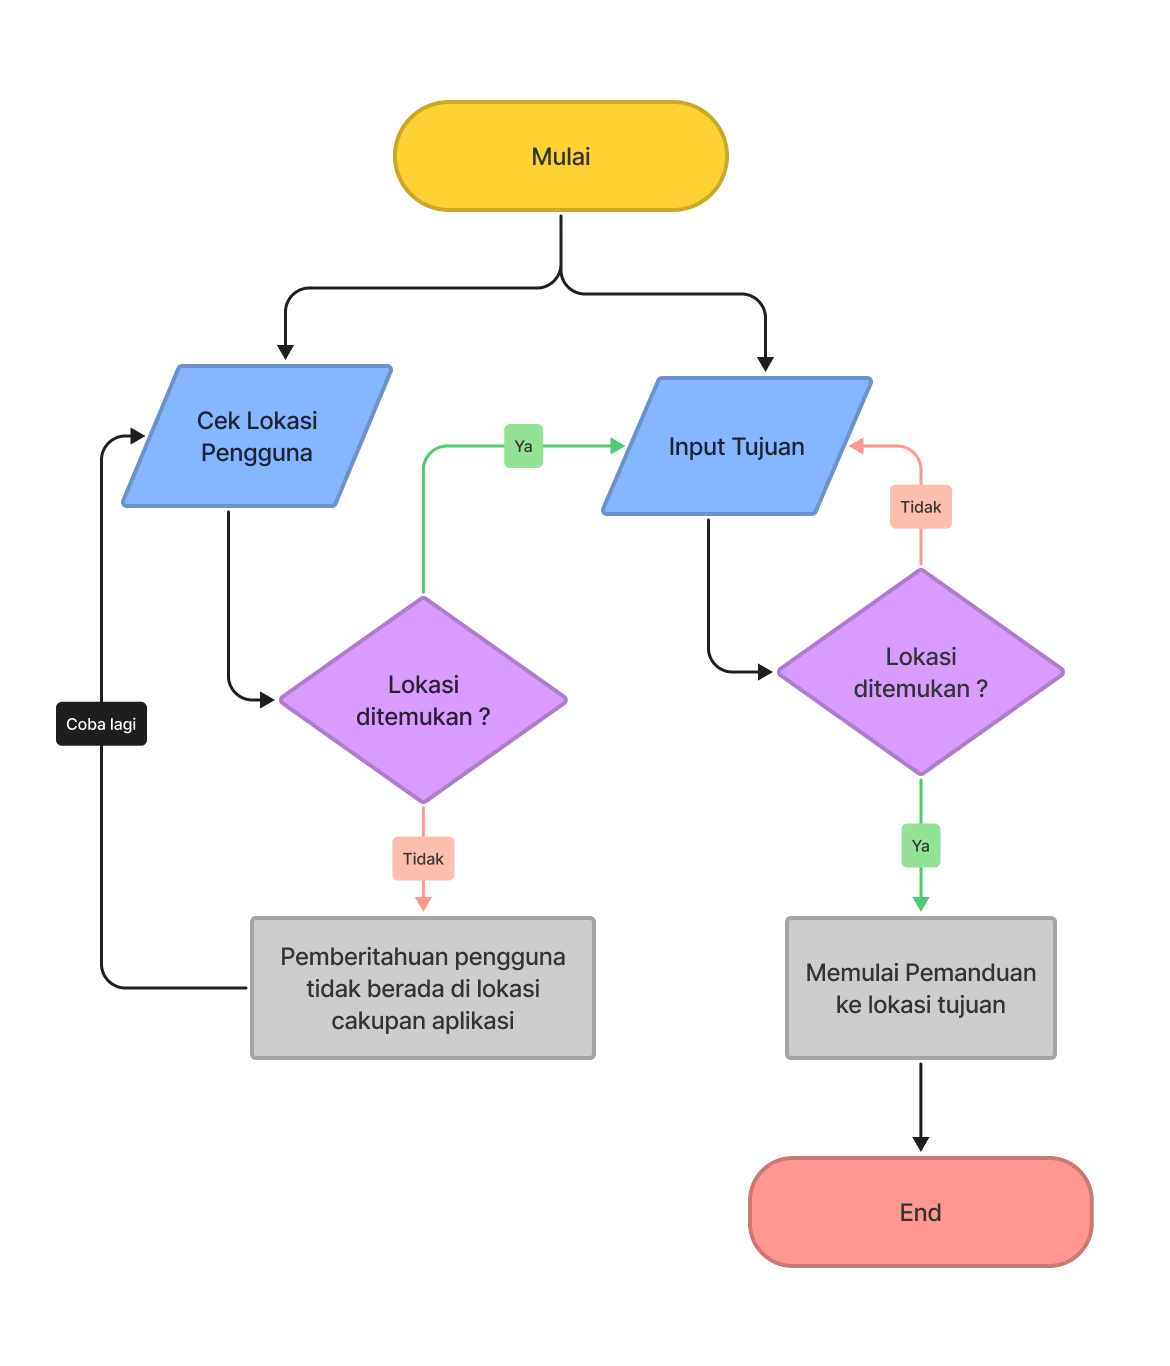
\includegraphics [scale = 0.35]{gambar/bab3/flow_diagram_app}}
\caption{\textit{Flow Diagram} Navigasi \textit{Indoor}}
\label{img:flow_diagram_app}
\end{figure}

\item Desain Prototipe
\par Desain prototipe menunjukkan perkiraan tampilan aplikasi yang akan dibuat. Desain ini dirancang berdasarkan beberapa skenario pada sisi pengguna baik tunanetra dan bukan tunanetra.

\vspace{-0cm}
	\begin{figure} [H]
	\begin{subfigure}{.5\textwidth}
  		\centering
  		% include first image
  		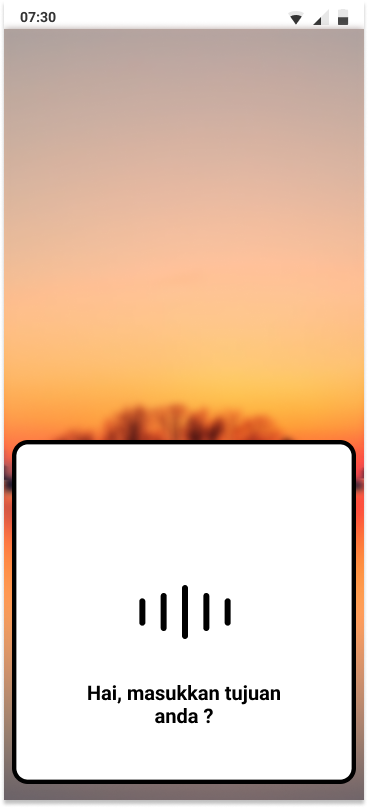
\includegraphics[width=.5\linewidth]{gambar/bab3/1}  
  		\caption{Pop up trigger by hotword}
	\end{subfigure}
	\begin{subfigure}{.5\textwidth}
  		\centering
  		% include second image
		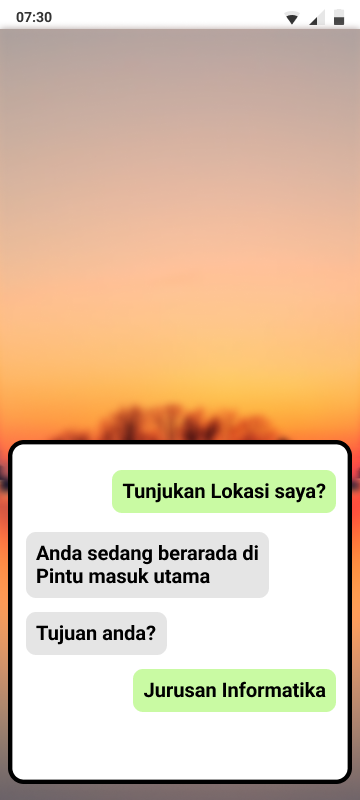
\includegraphics[width=.5\linewidth]{gambar/bab3/2}  
  		\caption{Input tujuan dan lokasi pengguna}
	\end{subfigure}
		\vspace{1cm}
		\newline
	\begin{subfigure}{.5\textwidth}
  		\centering
		 % include third image
	  	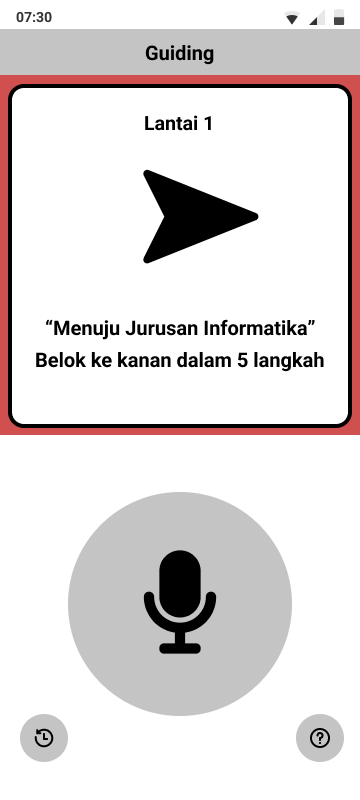
\includegraphics[width=.5\linewidth]{gambar/bab3/3}  
  		\caption{Proses Navigasi ke Tujuan}
	\end{subfigure}
	\begin{subfigure}{.5\textwidth}
  		\centering
  		% include fourth image
  		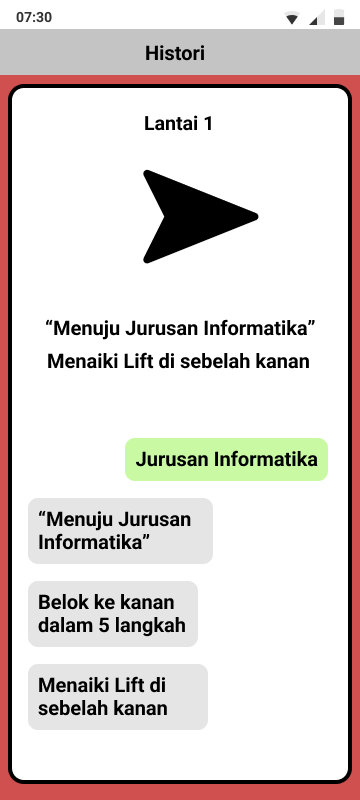
\includegraphics[width=.5\linewidth]{gambar/bab3/4}  
  		\caption{Histori Navigasi}
	\end{subfigure}
		\vspace{0.5cm}
		\caption{Tampilan Halaman Aplikasi Navigasi Indoor untuk Tunanetra}
	\label{aplikasimappingbagian1}
	\end{figure}

\end{enumerate}

%%%%%%%%%%%%%%%%%%%%%%%%%%%%%%%%%%%%%%%%%

\subsection{Pengumpulan Data}
\begin{enumerate}
\item Data Model \textit{Voice Recognition}
\par Data yang digunakan dalam penelitian ini terdiri atas data \textit{pre-trained} model yang diperoleh dari penelitian yang berada dalam satu penelitian yang sama pada \textit{roadmap} pada gambar \ref{img:fase2}. \textit{Pre-trained} model dimanfaatkan sebagai titik awal untuk merespons perintah suara dari pengguna, kemudian perintah suara akan di terjemahkan ke dalam bentuk teks yang akan diterima oleh \textit{smartphone} pengguna. Teks yang diterima akan digunakan sebagai input yang akan menjadi lokasi tujuan serta pemilihan rute.

\item Data Rute dan Denah Lokasi Penelitian
\par Rute yang akan digunakan berlokasi di gedung A FMIPA lantai 1 sampai dengan lantai 3. Data rute yang digunakan akan di petakan dengan menggunakan bantuan BLE. Data / titik-titik BLE disimpan dalam \textit{database} lokal berupa MAC \textit{Address}, nilai RSSI, dan nama perangkat BLE. Dengan adanya RSSI atau kekuatan sinyal yang disimpan perangkat smartphone pengguna akan menangkap sinyal dan menyesuaikan dengan titik-titik yang telah dipetakan sehingga mendapatkan lokasi pengguna berada serta menjadikan titik lokasi pengguna sebagai pemilihan rute terdekat ke lokasi tujuan pengguna.

\item Data \textit{Text-to-Speech}
\par Data yang akan digunakan menggunakan \textit{text-to-speech} yang disediakan oleh library Google speech. Sehingga proses pemanduan menuju ruangan akan dipandu dengan suara seperti "Menuju Ruangan Jurusan Informatika", "Belok ke kanan dalam 5 langkah", "Telah sampai di tujuan , Ruangan Jurusan Informatika".

\item Data akurasi lokasi pengguna serta akurasi rute
\par Data yang akan diperoleh dari proses koneksi BLE terdekat dengan RSSI sebagai tolak ukur akurasi lokasi pengguna, sedangkan untuk akurasi rute menggunakan data pemetaan rute dan lokasi tujuan yang telah dipetakan pada aplikasi dengan memanfaatkan RSSI dari beberapa koneksi BLE terdekat yang saling terhubung menggunakan Kalman Filter.

\end{enumerate}

\newpage
\subsection{Pembuatan Sistem Aplikasi}
Pada Proses pembuatan sistem aplikasi, metode pengembangan aplikasi yang digunakan adalah metode \textit{Scrum}, dikarenakan sistem ini dikembangkan bersama dengan tim dan membutuhkan fleksibilitas terhadap perubahan yang terjadi dalam proses pengembangannya, sehingga memerlukan iterasi secara berkala agar berjalan dengan baik. Salah satu tahap yang merupakan paling awal dari metode ini adalah \textit{product backlog}. Pada tahap ini, semua kebutuhan akan ditransformasikan menjadi rancangan pekerjaan untuk diselesaikan agar aplikasi dapat bekerja secara fungsional. Adapun \textit{product backlog} dari keseluruhan aplikasi ini adalah sebagai berikut.

\begin{itemize}
\item Menampilkan halaman beranda.

\item Menampilkan \textit{Pop up} yang muncul dari \textit{input} suara.

\item Meluncurkan aplikasi dengan proses pengenalan suara.

\item Menampilkan dan mengeluarkan suara daftar ruangan yang bisa di gunakan sebagai tujuan.

\item Menampilkan rute terdekat ke ruangan yang di tuju oleh pengguna.

\item Mengeluarkan suara navigasi ke ruangan yang di tuju.

\end{itemize}

\subsection{Pengujian Akurasi}
Pengujian akurasi posisi pengguna dan pemilihan rute akan menggunakan gabungan titik BLE sebagai titik awal dengan mengukur kekuatan RSSI, kemudian menggunakan letak dan posisi BLE yang telah dipetakan sebelumnya untuk melakukan pemilihan rute serta proses navigasi yang akan diprediksi menggunakan algoritma Kalman Filter disertai dengan fase pembaharuan prediksi titik lokasi pengguna ke tujuan.

\newpage
Berikut perhitungan yang akan digunakan untuk menguji akurasi pengguna serta rute pengguna, rumus menurut \citep{ihsan2018analisis}:
\begin{itemize}
\item \textit{Time Update (Predict)}

\par \textit{Predict State}
\begin{equation}
x = x
\end{equation}

\par \textit{Predict error covariance}
\begin{equation}
p = p + q
\end{equation}

\item \textit{Measurements update (Correct)}
\par \textit{Update the estimate via} k 
\begin{equation}
x = x + k*(measurement – x)
\end{equation}

\par Kalman \textit{gain} 
\begin{equation}
k = p / ( p+r )
\end{equation}

\par \textit{Update the error covariance}
\begin{equation}
p = (1 – k )* p
\end{equation}

\end{itemize}
\par Keterangan
\par x: Nilai yang di filter
\par p: Error estimasi
\par q: Noise yang diakibatkan dari proses
\par k: Kalman Gain
\par r: Noise dari sensor\newline

\subsection{Pengujian Fungsionalitas dengan Metode \textit{Black Box}}
Metode yang digunakan untuk melakukan pengujian fungsionalitas adalah dengan \textit{black box testing}. Pengujian ini dilakukan untuk memeriksa fungsi-fungsi pada sistem yang dibangun pada penelitian ini apakah sudah bekerja sesuai dengan kebutuhan pengguna ataupun tidak. Pengujian ini dilakukan dengan cara menjalankan setiap fungsi yang ada pada sistem dan memastikan agar sistem dapat bekerja dengan semestinya sesuai alur yang telah dirancang. Pengujian ini juga dapat melibatkan target pengguna dan pengembang.

\subsection{\textit{Usability Testing}}
\textit{Usability Testing} merupakan pengujian aplikasi untuk melihat apakah pengguna dapat dengan mudah dan nyaman dalam menggunakan aplikasi tersebut serta melihat dan mengevaluasi keberhasilan dari sebuah produk atau jasa. Pengujian ini akan menggunakan metode UMUX. UMUX terdiri dari 4 pertanyaan dengan menggunakan skala 1-7. Berikut daftar pertanyaan-pertanyaan dengan metode UMUX dapat dilihat pada Tabel \ref{tab:UMUX}.

\begin{table}[H]
\caption{Daftar Pertanyaan Metode UMUX.}
\label{tab:UMUX}
\resizebox{\columnwidth}{!}{%
\begin{tabular}{|l|l|}
\hline
1 & Kemampuan sistem ini memenuhi persyaratan saya.                  \\ \hline
2 & Menggunakan sistem ini adalah
pengalaman yang membuat frustrasi.  \\ \hline
3 & Sistem ini mudah digunakan.                                       \\ \hline
4 & Saya harus menghabiskan terlalu banyak waktu untuk
memperbaiki hal-hal dengan sistem ini. \\ \hline
\end{tabular}%
}
\end{table}

Untuk menghitung skor akhir metode UMUX \citep{finstad2010usability}, dapat dilihat dari cara berikut.

\begin{enumerate}
\item Item ganjil diberi skor [ skor pengguna - 1]. Item genap diberi skor [7 - skor pengguna].

\item Jumlahkan perbedaan ini dan bagi jumlahnya dengan 24 (skor tertinggi).

\item Kalikan hasil dengan 100.

\item Cari nilai rata-rata dari seluruh pengguna.
\end{enumerate}

\par Tingkat nilai skala pengujian menentukan apakah sistem tersebut layak digunakan, bermanfaat, diterima oleh pengguna dan bertahan lama penggunaannya. Sebuah sistem dengan nilai pengujian yang tinggi membuat sistem tersebut menjadi populer dalam waktu yang lama dan penggunaannya yang luas, dikarenakan banyak individu akan merasakan manfaat dari kehadiran sistem tersebut. Sedangkan sistem dengan nilai pengujian yang rendah, sering kali diabaikan walaupun dibuat berdasarkan kebutuhan dan menghasilkan sumber daya yang banyak.



%-----------------------------------------------------------------------------%

% Baris ini digunakan untuk membantu dalam melakukan sitasi
% Karena diapit dengan comment, maka baris ini akan diabaikan
% oleh compiler LaTeX.
\begin{comment}
\bibliography{daftar-pustaka}
\end{comment}